% This LaTeX was auto-generated from MATLAB code.
% To make changes, update the MATLAB code and export to LaTeX again.

\documentclass{article}

\usepackage[utf8]{inputenc}
\usepackage[T1]{fontenc}
\usepackage{lmodern}
\usepackage{graphicx}
\usepackage{color}
\usepackage{hyperref}
\usepackage{amsmath}
\usepackage{amsfonts}
\usepackage{epstopdf}
\usepackage[table]{xcolor}
\usepackage{matlab}
\usepackage[paperheight=795pt,paperwidth=614pt,top=72pt,bottom=72pt,right=72pt,left=72pt,heightrounded]{geometry}

\sloppy
\epstopdfsetup{outdir=./}
\graphicspath{ {./blocks_media/} }

\begin{document}

\begin{matlabcode}
g1 = tf(1, [1 10]);
g2 = tf(1, [1 1]);
g3 = tf([1 0 1], [1 4 4]);
g4 = tf([1 1], [1 6]);
h1 = tf([1 1], [1 2]);
h2 = 2;
h3 = 1;

gf1 = feedback(series(g3, g4), h1);
gf2 = feedback(series(gf1, g2), h2 / g4);
t = feedback(series(gf2, g1), h3);

t = minreal(t);
zpk(t)
\end{matlabcode}
\begin{matlaboutput}
ans =

                        0.5 (s+2) (s+1)^2 (s^2 + 1)
  -----------------------------------------------------------------------
  (s+9.914) (s+1.907) (s+1) (s^2 + 1.224s + 1.053) (s^2 + 5.954s + 18.39)

Continuous-time zero/pole/gain model.
Model Properties
\end{matlaboutput}
\begin{matlabcode}

figure;
subplot(2, 2, 1); step(t); title('Step Response'); grid on;
subplot(2, 2, 2); impulse(t); title('Impulse Response'); grid on;
subplot(2, 2, 3); bode(t); title('Bode Plot'); grid on;
subplot(2, 2, 4); pzmap(t); title('Pole-Zero Map'); grid on;
\end{matlabcode}
\begin{center}
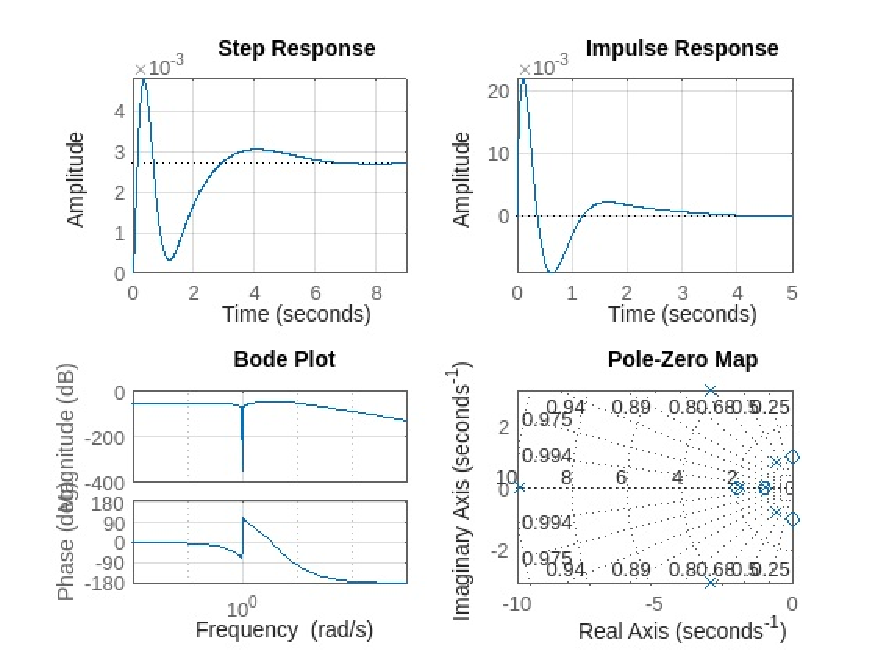
\includegraphics[width=\maxwidth{56.196688409433015em}]{figure_0.pdf}
\end{center}

\end{document}
